%%THIS IS A SHARED GDOC. DO NOT EDIT ANY LOCAL TEX FILE VERSIONS%%

\documentclass[conference]{IEEEtran}
\IEEEoverridecommandlockouts  
% The preceding line is only needed to identify funding in the first footnote. If that is unneeded, please comment it out.
%\usepackage{cite}
\usepackage{amsmath,amssymb,amsfonts}
\usepackage{algorithmic}
\usepackage{graphicx}
\usepackage{textcomp}
\usepackage{array}
\usepackage{tabu}
\usepackage{subfig}
\usepackage{todonotes}
\def\BibTeX{{\rm B\kern-.05em{\sc i\kern-.025em b}\kern-.08em
        T\kern-.1667em\lower.7ex\hbox{E}\kern-.125emX}}
\makeatletter

\onecolumn

\begin{document}
    
    \title{OpenPodCar: An Open Source Vehicle For Self-Driving Car Research }
    
    \author{
        Fanta Camara$^{1,2}$, \IEEEauthorblockN{Chris Waltham$^{2}$, David Churchill$^{2}$, Charles W. Fox$^{1,2}$}
        \IEEEauthorblockA{$^{1}$ Institute for Transport Studies, University of Leeds, UK}
        \IEEEauthorblockA{$^{2}$ School of Computer Science, University of Lincoln, UK}
   %     \IEEEauthorblockA{\IEEEauthorrefmark{3} Ibex Automation Ltd., UK}
    }    
    \maketitle
    
    
    \begin{abstract} 
Open source software for autonomous vehicle (`self driving car’) control is now available but there is a need for a corresponding open-source hardware platform to enable researchers to build standard setups and share research in this field.   Here we are constructing such a platform. The Lincoln OpenPodCar is a physical vehicle based on a low cost off the shelf, hard canopy, mobility scooter.  It is large enough to transport one person at speeds up to 15kmh, for example for use as a last-mile autonomous taxi service from the train station to the office; or to transport up to three Deliveroo-sized freight containers similarly around a city center. But it is also small enough to make serious injury to pedestrians unlikely in the event of a collision.  Together with its low costs it thus forms an ideal balance between real world utility, safety, cost and research convenience.  The open source platform consists of (a) hardware components: CAD designs, sample bill of materials, and build instructions to modify the off the shelf donor vehicle for electronic control; (b) Arduino, ROS and Gazebo control and simulation software files which provide standard ROS interfaces and simulation of the vehicle; and (c) higher-level ROS implementations of standard medium-level robot control, including the movebase interface which enacts command to get the vehicle from one pose to another. The vehicle uses Ackermann steering and Reeds-Sheppe curves. Its total build cost in 2022 is around 7000USD in total, including sensors and computing equipment.
    \end{abstract}    
    
    \begin{IEEEkeywords}
        Autonomous Vehicles,  Open Source Hardware and Software, Human-Robot Interaction.
    \end{IEEEkeywords}

\todo{Change Fig. 1 with a new one}    
    \begin{figure}[h]
      \includegraphics[width=\columnwidth]{hardware/testDrive.png}
      \caption{OpenPodcar test drive.}
      \label{fig:testDrive}
    \end{figure}




\section{Introduction}

Pick a licence for the paper github: e.g. CERN hardware licence

\subsection{Open source hardware}

The use of open source hardware (OSH) allows for more effective and accessible sharing and collaboration among researchers \cite{fisher2012open}, as well as more accessible entry-level projects such as examples from Oxer and Blummings (2009)\todo{who?}. OSH brings a number of benefits to a research community, as a common context for results and accessible platform with which to test new ideas allows for more engagement, leading to a more mature field of study.


It is currently almost impossible to build any large hardware design that does not incorporate non-open designs or make use of non-open designs as tools during construction. In contrast, open source simulation platforms are widely available for autonomous vehicle research, such as CARLA \cite{dosovitskiy2017carla}, SUMMIT \cite{cai2020summit}, FLOW\footnote{https://flow-project.github.io/}, DEEPDRIVE\footnote{https://github.com/deepdrive/deepdrive}, AirSim\cite{shah2017airsim}, LGSVL Simulator \cite{rong2020lgsvl} and Gym-Duckietown \cite{chevalier-boisvert2018duckietown}.

The podcar is currently only "weak" OSH, like the Arduino, because it depends on the use of a patented donor vehicle and uses sensors or other components e.g. 3D Lidar that are also patented. It is intended as a basis for future work which could replace the patented components with open interfaces to progress it to "deeper" OSH.
   

\subsection{Requirements}
Specific requirements for such a platform are that it needs to be as low cost as possible, and easy to build.  This is to enable the community to reproduce and use it. Consumer levels of safety and reliability are not required, preferring to minimise cost, though research standards of safety and reliability are required.
    
\subsection{Donor vehicle base}    
A Pihsiang TE-889XLSN hard-canopy scooter (branded in UK as Shoprider Traverso, \cite{shoprider2006}) is used as the podcar platform. It is an electric mobility scooter powered by two 12V batteries connected in series to provide 24V operating voltage and containing 75Ah. In its standard configuration, the donor vehicle’s steering is controlled by a human operated loop handle bar. The speed and braking systems are both powered by an electric motor and an electric brake via the trans-axle assembly, controlled by an AC2 digital controller receiving different voltage signals to drive forward or brake. The manual speeding and braking systems are controlled by three buttons connected in series on the handle bar.  A toggle switch in parallel with a resistor (10k$\Omega$) to choose speed mode high or low; A speed dial knob via a variable resistor (20k$\Omega$) to choose a maximum speed value; A throttle lever connected with a potentiometer (5k$\Omega$), 2.5k$\Omega$ to 2.6k$\Omega$ for each side to speed or brake. 

\subsection{Open source software base}

ROS, is `an open source operating system' for robots based on a publish-subscribe pattern \cite{quigley2009ros}, which is the robotics community’s standard interface. Building on top of ROS, the `ROS ecosystem’ is a loosely-defined collection of open-source ROS packages with variously accepted standard message formats which act as conventional interfaces to enable many community packages to work together and to act as swappable alternatives for one another.   

ROS drivers are packages in the ecosystem which wrap robot hardware with standard ROS interfaces.

ROS launch files are stored configurations of ROS nodes that can be run using one command from a terminal. These are used widely by ROS packages to quickly launch the nodes required for a certain task at the same time.

tf is a ROS ecosystem library for 3D transforms. Transformas are a substantial part of ROS that allows for sensor input and other systems that require spatial frames to be contextualised by the sensors relative position within the robot. These are published on the ‘tf’ topic, as explained by Quigley et al (2009), and create “a dynamic transformation tree which relates all frames of reference in the system” .

Gazebo \cite{koenig2004design} is a robotics 3D physical simulation and 3D graphics display tool, separate from, but designed to integrate with ROS, and which is the robotics community standard simulator.  An example of one such project that makes use of Gazebo in conjunction with ROS is reported by Qian et al 2014) which presents an example of a project in which the hardware and software are developed in parallel, making use of ROS (for providing the software interface) and Gazebo (for testing hardware that doesn’t yet exist in the real world). 

\subsection{Path planning and control}

Path planning means the selection of an entire desired trajectory for a robot to get from a current pose to a desired pose, where a pose is a position together with a heading direction.  Path planning may be split into high level and local planning, where high level makes large scale decisions such as which way to go around obstacles, while local planning refines these choices into specific curves with optimal properties. Path control (or path following) is then the real-time process of executing a path plan by interactively monitoring the robot’s state, sending commands to motors, and trying to make the actualized path as close to the desired path as possible.  

Movebase (wiki.ros.org/move\_base) is a ROS community standard which defines a set of message formats and a framework of ROS nodes for path planning and control.  This framework allows different algorithms to plug in to it.   Timed Elastic Band (TEB) \cite{rosmann2013efficient} is a local planner algorithm which has been integrated as a movebase plugin (wiki.ros.org/teb\_local\_planner).

Planning and control for car-like vehicles with a steering column is more complex than for differential drive (skid steer) vehicles which turn by having the wheels on one side rotate faster than the other. This is because differential drive vehicles are holonomic, meaning that in the absence of obstacles, they can move greedily from any pose to any other, while steered vehicles and non-holonomic, meaning that greedy motion is not guaranteed to reach a target pose and longer-term plans must be considered.    The shortest possible path for a forward-driving steered vehicle is the Dubins path \cite{dubins1957curves}, which always consists of two circle arcs connected by a straight line, which is generalized to the Reeds-Shepp path when reversing is also allowed \cite{reeds1990optimal}. Parallel parking is a classic difficult path planning task for Reeds-Shepp vehicles.

\subsection{Simulateneous Localisation and Mapping}
Simultaneous Localisation and Mapping (SLAM) \cite{thrun2002probabilistic} is the robotic task of inferring the robot’s location at the same time as building a map of its environment, which is a classic `chicken and egg’ problem as the two subtasks depend on one another. Solving SLAM is an NP-hard problem but many standard approximations exist. gmapping \cite{yuen2017improved} is a ROS implementation of a Rao-Blackwellized Particle Filter (RBPF)for 2D SLAM, in which “each particle carries an individual map of the environment”  The information carried by each particle overlaps, and an estimation of a map can be built based on these relationships. As the robot moves around the environment, these estimations are stored, and when a ‘feedback loop’ is closed, the estimations cascade into a portion of the completed map. These maps take the form of 2-D occupancy grids, and can be used later by the navigation stack to plan paths around the environment.

Performing SLAM in 3D is more computationally challenging, but has recently become possible due to hardware acceleration provided by parallel GPU computers.
OrbSLAM is a ROS 3D SLAM based on the Octomap algorithm, which can operate with mono visual features, or lidar or stereo camera point clouds. It maintains a voxel based map of the environment (similar to maps in the game Minecraft) and is a 3D analog of gmapping.

NDT SLAM  (used in Autoware and ILIAD) is another 3D SLAM implementation and algorithm based on Normal Distribution Transforms \cite{einhorn2015generic}.

\section{Related systems}

SMART [CITE] is a design to modify an existing donor golf cart vehicle for automation research, developed by MIT and Singapore.  The vehicle is a similar size and power to OpenPodCar but is not open source.
Beetlebot \cite{beetlebot} is a OSH system similar to OpenPodCar but for last-mile freight delivery, without human carrying capacity, and including ROS integration.
Open Source Ecology (OSE) [CITE??] is an ambition project which ultimately aims to develop Deep OSH vehicles including a car and tractor, via a process of progressively deeper Shallow OSH designs.  OSE is optimised for reliability and for users in developing countries so uses hydraulic power rather than electric as used in OPenPodCar.
Several functioning OSH designs for large cars exist, including Apollo\footnote{https://github.com/ApolloAuto/apollo}, PixBot\footnote{https://gitlab.com/pixmoving/pixbot} and OSVehicle Tabby \footnote{www.openmotors.co/tabbyevo/}.  AutoRally\footnote{https://autorally.github.io/} \cite{goldfain2019autorally} developed researchers at Georgia Tech and the Berkeley Autonomous Race Car (BARC\footnote{www.barc-project.com/}) are small-scaled autonomous vehicles for research, but only BARC includes ROS integration. 
 
Autoware \cite{kato2018autoware} is a heavyweight open source software project to construct a ROS based automation stack for large on-road cars with power on-board computers.
The state of Georgia, in the USA, provides a level 3 open-source autonomous vehicle based on a Ford-Edge at the Curiosity Lab at Peachtree Corners \footnote{https://www.peachtreecornersga.gov/businesses/curiosity-lab-at-peachtree-corners}, where technologists and researchers can use the platform in the smart city environment free of charge.


OSH and OSS are inherently cooperative design processes and legal structures, so it is possible that components from all of the above and from podcar will be interchanged and evolve together in the future.

https://ieeexplore.ieee.org/document/8926794


https://ieeexplore.ieee.org/document/8813784

 
\section{Mechanical modification}

\subsection{Steering}
To automate steering, a Gimson GLA750-P 12V DC linear actuator with position feedback is mounted between an anchor on the underside of the chassis and the car's front axle via bearings.  This actuator has a 8mm/s full load (750N) speed and 250mm stroke length (installation length is 390mm).  

To access the underside of the vehicle, use two axle stands as in fig. \ref{fig:axelStands}. There is an existing hole in the right front wheel axle.  Mount the linear actuator via rear hole to the left side of the front chassis and connect it through the front hole of the actuator with the hole in the car's right front wheel axle via bearings as shown in fig. \ref{fig:steering} and fig. \ref{fig:actuatorMounted}.

    \begin{figure}[h]
      \includegraphics[width=\columnwidth]{hardware/onAxles.jpg}
      \caption{Tilting the vehicle using two axle stands, to enable access to the underside. (Note also lidar mounted to roof.)}
      \label{fig:axelStands}
    \end{figure}

\begin{figure}[h]
      \includegraphics[width=\columnwidth]{hardware/steering1.png}
      \caption{The bottom view of front wheels steering relationship including geometric coefficients}
      \label{fig:steering}
    \end{figure}
    

    \begin{figure}[h]
      \includegraphics[width=\columnwidth]{hardware/steeringActuatorMounted.jpg}
      \caption{Underside with linear actuator added for steering.}
      \label{fig:actuatorMounted}
    \end{figure}

\subsection{Sensor installation}
\subsubsection{Lidar option}
A Velodyne16 lidar sensor is mounted on the vehicle roof using a small optical tripod (TODO give model). Note that optical devices have unusual physical mounting standards which use Imperial rather than metrics units.  This system is used by optics research based on optical table sizing.   The lidar screws onto the tripod. The tripod is cabled-tied to the vehicle roof via  drilled holes at locations in fig. TODO.  It is mounted at a 10 degree tilt downwards (to allow pedestrians to be most clearly seen in the 16 scan lines).

\subsubsection{Depth camera option}
A lower cost alternative to lidar is to use a stereo camera for point cloud sensing. In this option, a StereoLabs ZedCam is mounted similarly on the vehicle roof.

\subsubsection{TODO Odometry}
TODO -- we need some Hall effect or other shaft encoders to measure odometry.


\section{Electronics and Firmware}

\subsection{Initial design}

New vehicle electronics are added on an acrylic board mounted under the seat of the vehicle, as shown in fig. \ref{fig:circuitDiagram} and \ref{fig:actuatorMounted} and mounted as in fig. \ref{fig:actuatorMounted}. Details are described below.  Where different voltage power supplies are required, DCDC converters are used and mounted in the same way.

    \begin{figure}[h]
      \includegraphics[width=\columnwidth]{hardware/pic_boards.jpg}
      \caption{Below-seat area inside cabin, with newly added boards..}
      \label{fig:actuatorMounted}
    \end{figure}

    \begin{figure*}[h]
      \includegraphics[width=\linewidth]{hardware/circuitDiagram.png}
      \caption{Circuit diagram for electronic modifications.}
      \label{fig:circuitDiagram}
    \end{figure*}
    
    \begin{figure*}
    	\centering
    	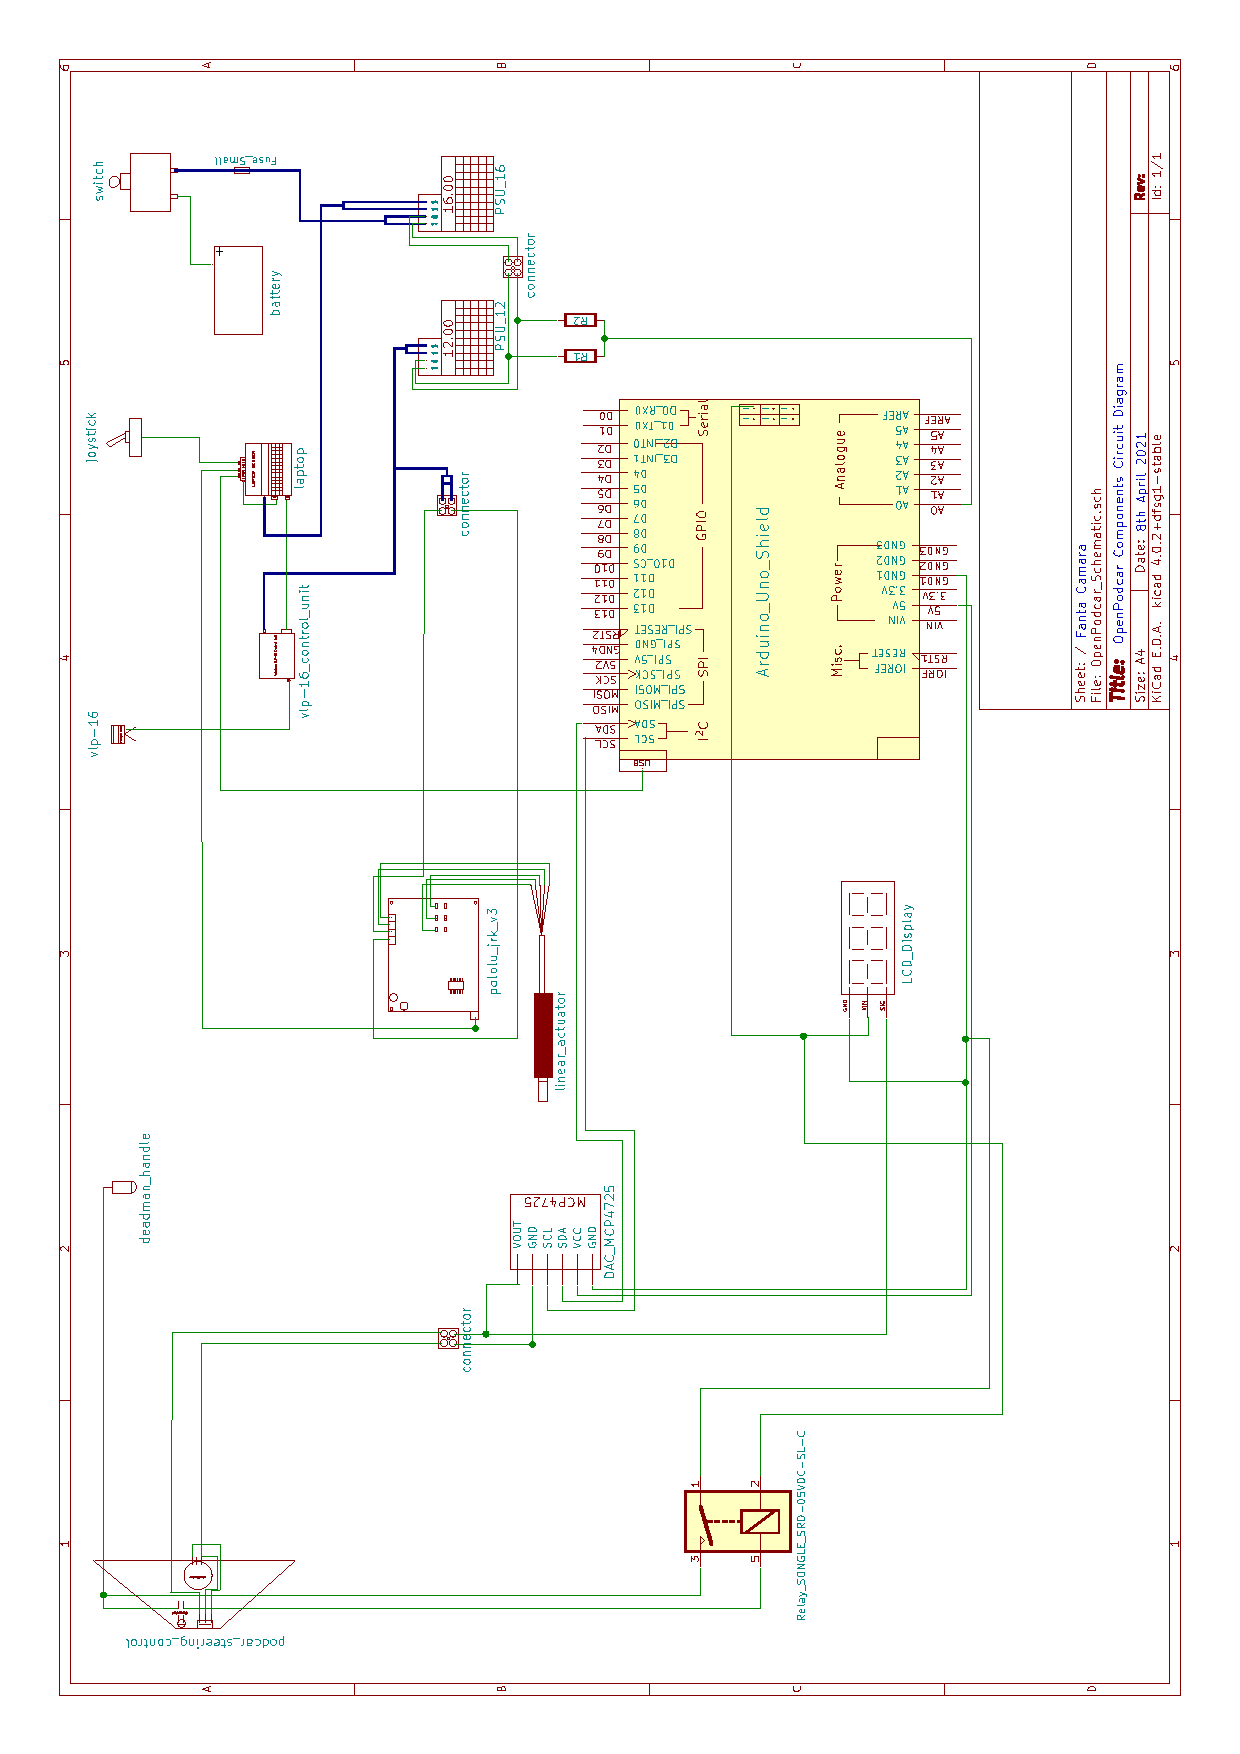
\includegraphics[width=0.9\linewidth]{hardware/OpenPodcar_Components_Circuit_Diagram_colored.pdf}
    	\caption{Complete Circuit Diagram for electronic modifications.}
    	\label{fig:CompleteCircuitDiagram}
    \end{figure*}
    
    \begin{figure}[h]
      \includegraphics[width=\columnwidth]{hardware/drilling.png}
      \caption{Drilling.}
      \label{fig:drilling}
    \end{figure}
    
   \subsection{PCB design}

	To robustify the initial electronics modifications, we further designed a PCB (Printed Circuit Board). The PCB is composed of two DC-DC Buck converters with XL4016 regulator, an Arduino Uno, a MCP4725 DAC (Digital-Analog Converter), a Pololu JRK 21v3 motor controller with position feedback, 2 resistors. We 3D printed parts to support the mounting of the LCD and the 3D LIDAR.  
	
	
	\begin{figure}[h]
		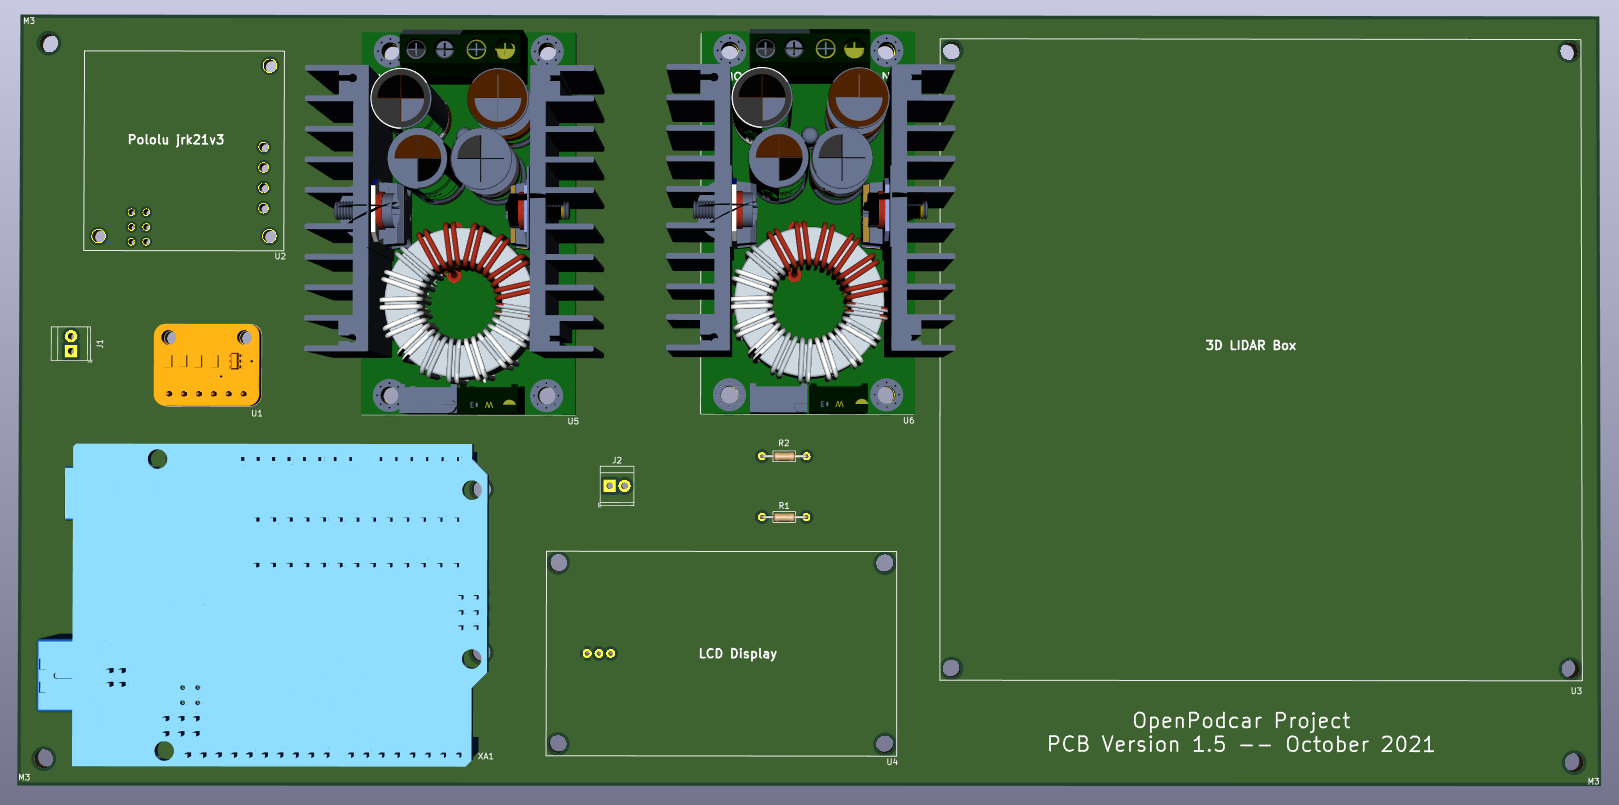
\includegraphics[width=\columnwidth]{hardware/pcb_version_1_5_pic1.png}
		\caption{PCB Design.}
		\label{fig:pcb_design}
	\end{figure}
	
	
	\begin{figure}[h]
		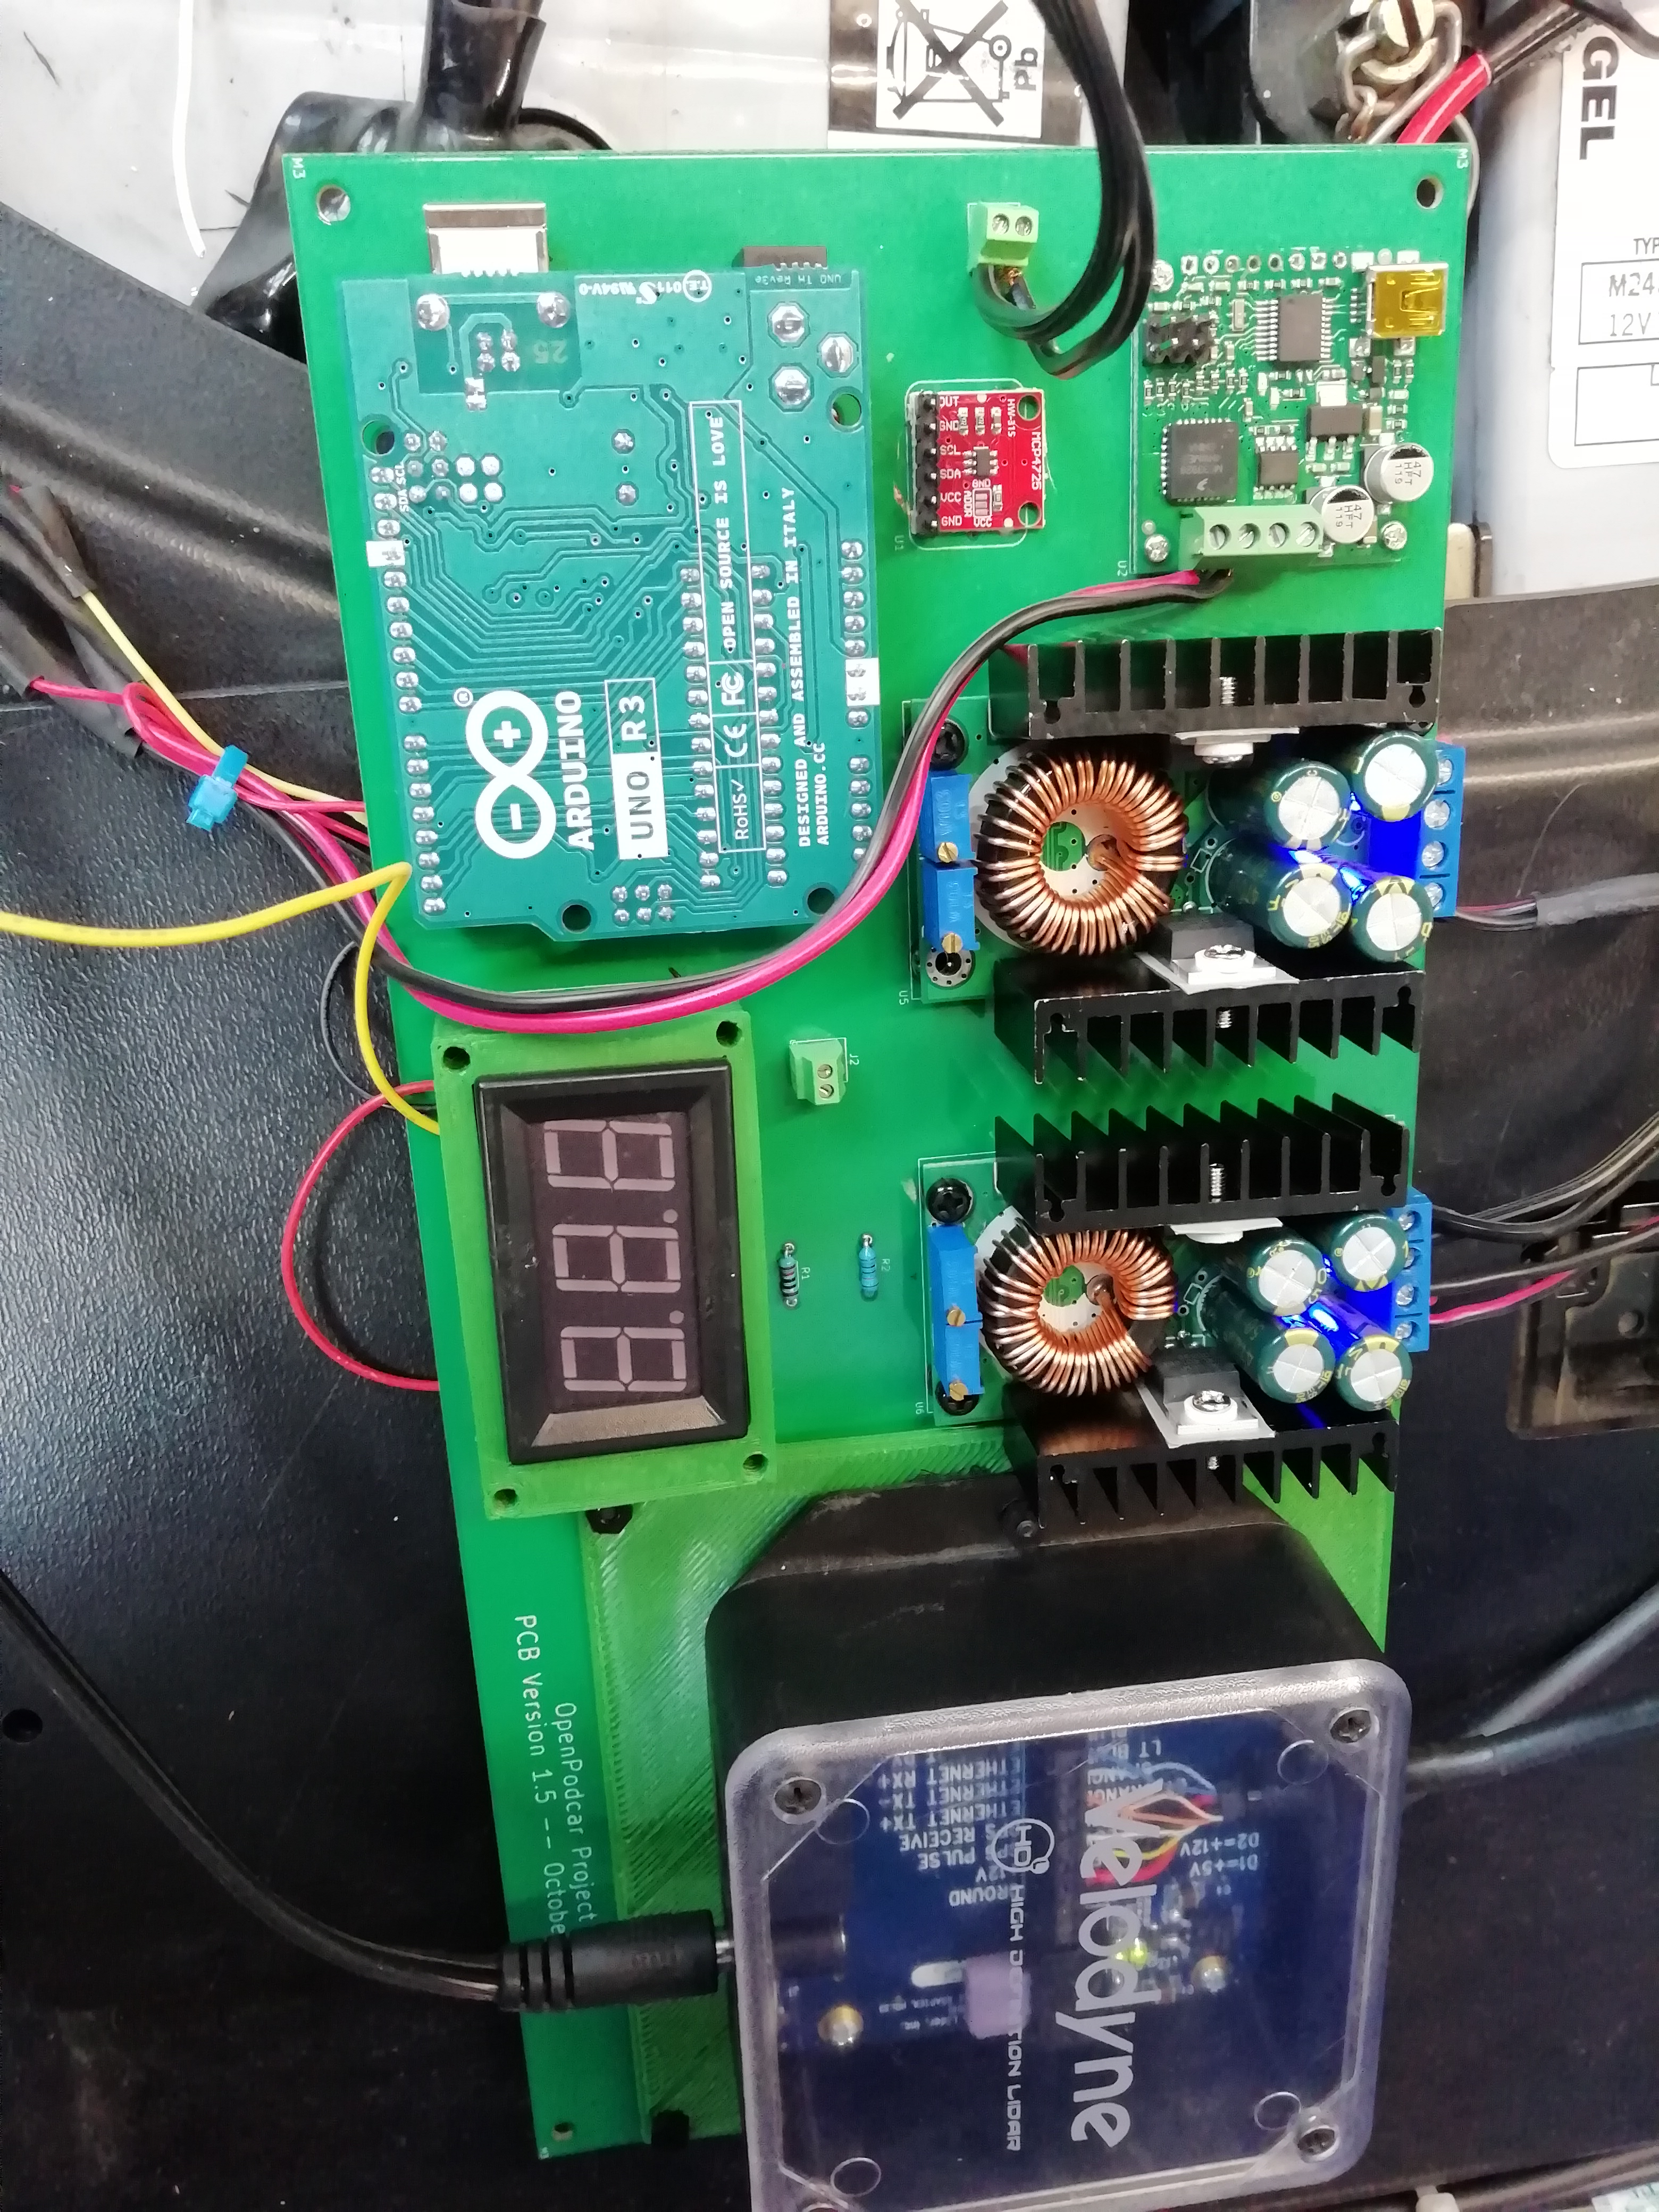
\includegraphics[width=0.75\columnwidth, angle=90]{hardware/pcb_podcar.jpg}
		\caption{PCB assembled.}
		\label{fig:pcb_assembled}
	\end{figure}

	

\subsection{Steering control system}

The front wheels are steered by a Pololu JRK21v3 PID controller, which takes serial port desired positions as input. It also takes feedback position information as an analog voltage from the linear actuator as an input. It outputs analog high-power voltages to the linear actuator.

TODO give PID settings.Windows app is needed to set them once only. 



The relationship between the required central turning angle $\theta$ of the pair of front wheels and extending length $l$ of linear actuator is,    
    \begin{gather}
    \theta = \alpha - \arctan(\frac{W}{2H}) \\
    % update W and H in figure. W is the width between two front wheels and H is the distance between front wheel and rear wheel.
    \beta = \alpha -\frac{\pi}{2}\\
    x = r_1 * \cos(\beta) \\
    y = r_1 * \sin(\beta) \\
    l = \sqrt{(x_0-x)^2 + (y_0-y)^2} - L + l_0    
    \end{gather}    
    Where $r_1$, $x_0$, $y_0$, $W$, $H$ and $L$ are the geometric coefficients shown in Fig.1. Among them, the value of $y_0$ is negative. $l_0$ is the initial value of the linear actuator position feedback.

    % related to:
    %'889XLSBN CAN Traveso Spare Parts List' page 29, 30, 32, 33, 34, 37, 38, 40 and 41;
    %'Shoprider Scooter Service Manual Live Document' page 7, 8, 14 and 16.

Diagnostic test commands can be passed to the Polulo using the commands provided in /tools/cmdSteer.   {\em Do not give commands outside the range 1000-25000 as they have damaged the vehicle.}  

TODO -- WRITE SAFETY WRAPPER TO LIMIT THIS RANGE..

A non-ROS test of the C API for the Pololu is provided in /tools/pololuTestCSerial.    

    \begin{center}
        \begin{tabular}{ c c }
            \hline
            FA:cmd     &  Effect \\
        2500    &    max right  \\
        1900    &    center  \\ 
        1000    &    max left  \\
            \hline\\
        \end{tabular}
    \end{center}    

 {\em Do not give commands outside this range as they have mechanically destroyed the system.}  

    
\subsection{Speed control system}

\subsubsection{Safety system}

Autonomous vehicles can present a significant hazard to people and the environment in which they operated. Damage to surroundings and possible injury to operators and bystanders could result from inappropriate use or malfunction. It is essential that a suitable emergency stop system is implemented in all autonomous vehicles.   Given the development platform nature of the OpenPodCar, a safety mechanism which stops the vehicle under fault conditions is an especially important part of the design.   The design thus requires a series of positive heartbeat signals to be present and timely and also a dead-mans handle (DMH) to be depressed by a human experimenter at all times, in order for a hardware relay to actively continue to supply power from the vehicle’s batteries to all other systems.  The relay will naturally cut out if these signals are absent for any reason, including failures in the safety systems themselves.

Implementing and testing this safety system should be undertaken with the drive wheels of the vehicle raised off of the ground, allowing for checks to be made of the DMH without the risk of the vehicle speeding off out of control.

The speed controller on this particular mobility scooter has a dead zone at around 2.5V on its speed input signal which corresponds to drive wheels stopped. Above the dead zone and up to 5V being forward control values and 0V to below the dead zone being reverse control voltages.

These values were checked using a multi-meter prior to implementing the Arduino controller and DAC.  This means that if the DAC output from the Arduino where to fail and 0V for example is applied to the mobility scooters speed controller input, the vehicle would respond by spinning the drive wheels backwards at full throttle. This being a dangerous eventuality, it is very important in terms of safety to ensure this situation can not arise.

A two stage approach is used to reduce this risk. Refer to the schematic diagram DMH section in conjunction with this description.

\paragraph{Stage 1 – Relay.} A relay is used which interrupts the mobility scooter’s key ignition circuit. If the relay is not energised by the presence of a 5V supply to the Arduino, the vehicle’s movement is disabled. This effectively ensures that if the Arduino is non-functional, for example its power supply has failed or it has been unplugged from the USB port of the control PC and there is a danger that the DAC is not producing the control systems required voltage, the scooter is automatically disabled by effectively switching it off.

\paragraph{Stage 2 – DMH Switch.} A sturdy push button is used which also interrupts the vehicle's key ignition circuit. If the PodCar operator detects any abnormality in operation during operation, he/she simply releases pressure from the DMH switch and the vehicle’s movement is disabled. The DMH switch is wired in series with the relay in the key ignition circuit ensuring that if both the relay contacts and the DMH switch are closed, this is the only condition where the PodCar movement is active.

The addition of the Relay and the DMH Switch are essential for safe operation, especially where new unproven autonomous control systems are in development.

A photograph of the installed system is shown in fig. \ref{fig:actuatorMounted}.

    \begin{figure}[h]
      \includegraphics[width=\columnwidth]{hardware/pic_relay.jpg}
      \caption{Steering console showing newly added relay (with lit LED) to dead man’s handle, replacing the ignition switch (only) in the circuit.}
      \label{fig:actuatorMounted}
    \end{figure}

Deadman’s handle to ignition. Replace key with relay (TODO model) and dead-mans-handle button switch (TODO model) on a 10m, 2-core cable.    TODO: are any other console functions changed? 

TODO edited version of wiring from shoprider manual. And photo of the real wires.

TODO how to set the console switches to correct fixed settings.


\subsubsection{Speed controller}

An Arduino UNO \cite{oxer2011practical} is used to send electric signals to the vehicle's motor controller in place of the donor vehicle’s paddle controller’s potentiometer.    An Adafruit MCP4725 DAC is connected to the Arduino as in fig. \ref{fig:circuitDiagram}, and used to send clean analog speed command voltages to the donor vehicle’s internal controller.

Arduino code is supplied in the distribution (/Arduino/ThrottleControlSerial.ino). When uploaded to the Arduino (using the standard Arduino IDE running on the laptop), it provides a simple serial port API running at 112000baud (TODO other erial options.)  It receives commands of the form “FA:210” as speed commands.   The test scripts /tools/zeroSpeed.py and /tools/testSpeed.py can be used to send example commands for debugging.

    \begin{center}
        \begin{tabular}{ l c c }
            \hline
        Command   &    Voltage            &  Effect \\
        FA:0      &    0                  & stupid fast reverse  \\
        FA:80     &    $\sim 0.9$         & v fast reverse (ros limit) \\
        FA:132    &   $\sim 1.5$          & slowest reverse motion  \\
                  &                       & dead zone - allows ignition \\
        FA:170    &    1.9                & stop - zero/home position \\
        FA:201    &    $\sim 2.3$         & slowest forward motion \\
        FA:240    &    $\sim 2.7$         & v fast forward (ros limit) \\
        FA:255    &    $\sim 3.0$         & stupid fast forward \\
            \hline\\
        \end{tabular}
    \end{center}    

To start the ignition, the car safety system requires the control voltage to be in the dead range.   A problem is that this doesn’t correspond precisely to any fixed speed bytes, due to the USB power issues.  But if we pick a number solidly in the center of the dead zone, such as 164, this will work for most USB supplies.   (i.e. when the vehicle’s battery is flatter, the voltages provided to USB power by it are lower. For example, we might send 164 and get 1.9V instead of the usual 2.26V.)   This may result in the vehicle not starting - maybe by design or accident. (This produces a beep as is outside the start zone.)  The Arduino is getting lower power eg max 4.9V instead of 5V, which gets divided by the DAC value.  To deal with these instabilities, we added a potential divider at the battery to check the voltage and control the podcar accordingly, as in Fig. \ref{fig:potential_divider}. We provide a “BV” command in the Arduino serial protocol which allows callers to request the current battery voltage. This can then be used by the higher level (Python) systems to decide what speed bytes to sent, including compensating for the floating dead zone.

      \begin{figure}
      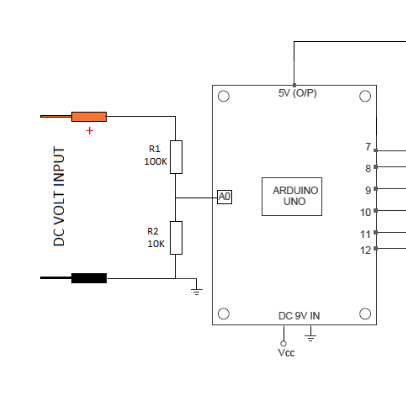
\includegraphics[width=\columnwidth]{hardware/potential_divider.png}
      \caption{Potential divider linked to the battery}
      \label{fig:potential_divider}
    \end{figure}

\section{Physical vehicle software interface (ROS)}

A ROS interface to and from the physical vehicle is provided as illustrated in fig. \ref{fig:meshSim} and described below. This runs on a Panasonic CF-19 Toughbook computer mounted on-board the vehicle (and powered from a DCDC converter from the  vehicle battery) running Xubuntu 16.04 (Xenial) and ROS Kinetic.

\begin{figure*}[h]
      \includegraphics[width=\textwidth]{software/rosnodes.png}
      \caption{ROS nodes and messages for low-level control.}
      \label{fig:meshSim}
\end{figure*}

\subsection{Control system interface}
The system expects to hear two incoming ROS control messages:     speedcmd\_meterssec and wheelAngleCmd, which contain single floats representing the desired speed in meters per second, and the desired front wheel orientation in radians respectively.

These two messages are received by ROS nodes speedm2arduino and wheelAngle2Pololu, which are ROS drivers for the Arduino speed controller and the Polulo steering controller respectively.

\subsection{Manual joystick control}
Converters from a standard ROS USB joystick driver node to the speed and angle command interface messages are provided, by joystick2speedms and joystick2wheelAngle.  These use the $y$ axis of a joystick for speed and $x$ for steering.

\subsection{Lidar option}
Velodyne works with the velodyne ROS package. But it needs to be set up so we can talk to the Velodyne over ethernet.  The laptop must be on a wired network, not wifi.   The IPs must be configured as in the velodyne docs TODO details/refs.  The lidar IP is 192.168.1.201.

\section{Simulation}

\subsection{Podcar 3D Sim}

    \begin{figure}
      \includegraphics[width=\columnwidth]{software/podcar_phys_sim.png}
      \caption{Physical simulation of vehicle.}
      \label{fig:physSim}
    \end{figure}

    \begin{figure}
      \includegraphics[width=\columnwidth]{software/podcar_mesh.png}
      \caption{Visual mesh simulation of vehicle.}
      \label{fig:meshSim}
    \end{figure}

A robotics simulation of the vehicle is provided for use in Gazebo 8.6.0 under ROS Kinetic and Ubuntu 16.04 (Xenial).

\todo{Change Fig. 14 with a real physical simulation of the vehicle} 

The physics simulation is based on a simplified vehicle geometry with two large cuboids containing the vehicles’ mass. \ref{fig:physSim} Parallel steering linkage is simulated via ODE joints forming a tracking rod. Rear drive motor and the steering linear actuator are simulated via ODE PID controllers.  Wheel geometry was measured from the physical vehicle.   Wheel forwards and lateral Coulomb friction coefficients were tuned by trial and error to produce realistic motion and steering.  The model is represented in SDF format, which is easy portable for use in other simulation and CAD systems.

There are some key differences when it comes to actuating the tracking rod between simulation and real life. On the physical robot, a linear actuator is mounted on the underside of the vehicle and attached to the front axle, which can extend/retract to angle the wheels. However, in simulation, the pivot joints that join the front wheels and the tracking rod can have a force applied directly to them without the need for a complicated actuator. This reduces the complexity of the model without affecting its behaviour, and is still appropriately accurate to real life.

There are also some similarities, for example both steering solutions implement a PID
(Proportional, Integral, Derivative) controller, that uses a proportional gain, integral function
and differential function to determine exactly how much force to apply at any given time in
order to keep the wheels at the desired angle. The parameters for the existing robot’s PID
controller have not been published, however trial and error found a proportional gain of 2,
differential weight of 1 and integral weight of 0 were adequate.

The simulation implements the same ROS interface as the physical vehicle system to enable plug and plug interoperability between them.  In the simulation, vehicle control messages are received, and vehicle sensor messages are sent by, a Gazebo plugin (podcarGazeboROSPlugin.cpp) which calls Gazebo’s simulation functions.  

Desired vehicle control commands, as for the physical vehicle, consist of (speed, angle) pairs, to command the speed of the rear wheels in m/s (speedcmd\_meterssec message) and the steering angle (wheelAngleCmd message) of the front wheels in radians.  The plugin and Gazebo implement these commands using simulated rotary and linear PID controllers and actuators, to rotate the rear wheels and linearly actuate the tracking rod respectively.

The plugin then publishes sensor messages corresponding to those from the physical vehicle. These include:  /odometry/groundTruth, a (noiseless) standard odometry format estimate for the vehicle’s pose; and /camera/image\_raw and /camera\_depth, the depth camera data.

A detailed graphical mesh model of the vehicle is provided for display, rather than physical simulation, purposes \ref{fig:meshSim}.  This may be important for experiments such as virtual reality interactions between the simulated vehicle and human subjects, e.g. \cite{camara2021evaluating}, as their psychological responses may depend on the apparent size and share of the vehicle.

A basic 3D world containing the podcar and various test objects from Gazebo libraries is provided by default as shown in Ffg. \ref{fig:sim_world}.

Fig. \ref{fig:sim_nodes} shows the complete ROS node configuration used during simulation, under manual joystick control.  
\begin{figure}[h]
      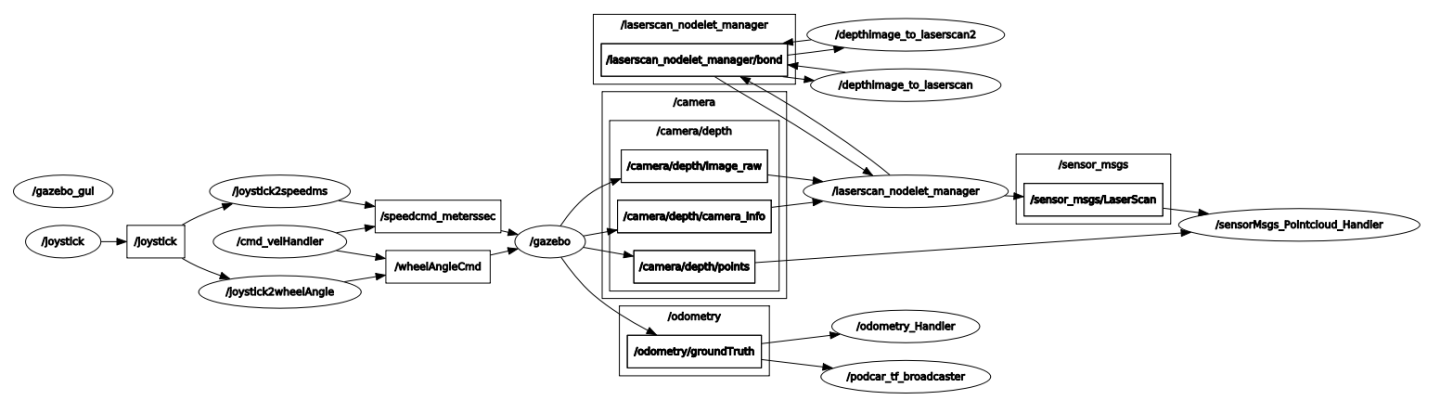
\includegraphics[width=\columnwidth]{figs_sim/sim_nodes.png}
      \caption{ROS nodes used in simulation under manual joystick control.}
      \label{fig:sim_nodes}
\end{figure}

\begin{figure}[h]
      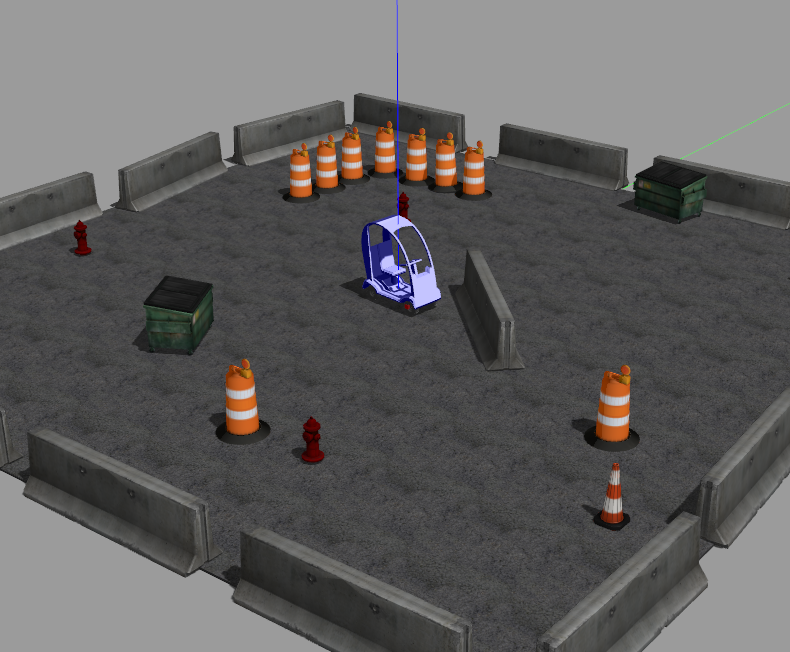
\includegraphics[width=\columnwidth]{figs_sim/podcar_loaded_gazebo.png}
      \caption{Initial gazebo simulation world}
      \label{fig:sim_world}
\end{figure}

	\subsection{University of Lincoln 3D Map}
	
	We used the open source Blender 3D add-on called MapsModelsImporter [CITE] to create a 3D world representative of the University of Lincoln campus, the testing area for the podcar. Before using MapsModelsImporter, RenderDoc [CITE], a free graphics debugger, is used to capture 3D data from Google Streetviews.  
	
	\begin{figure*}[h]
		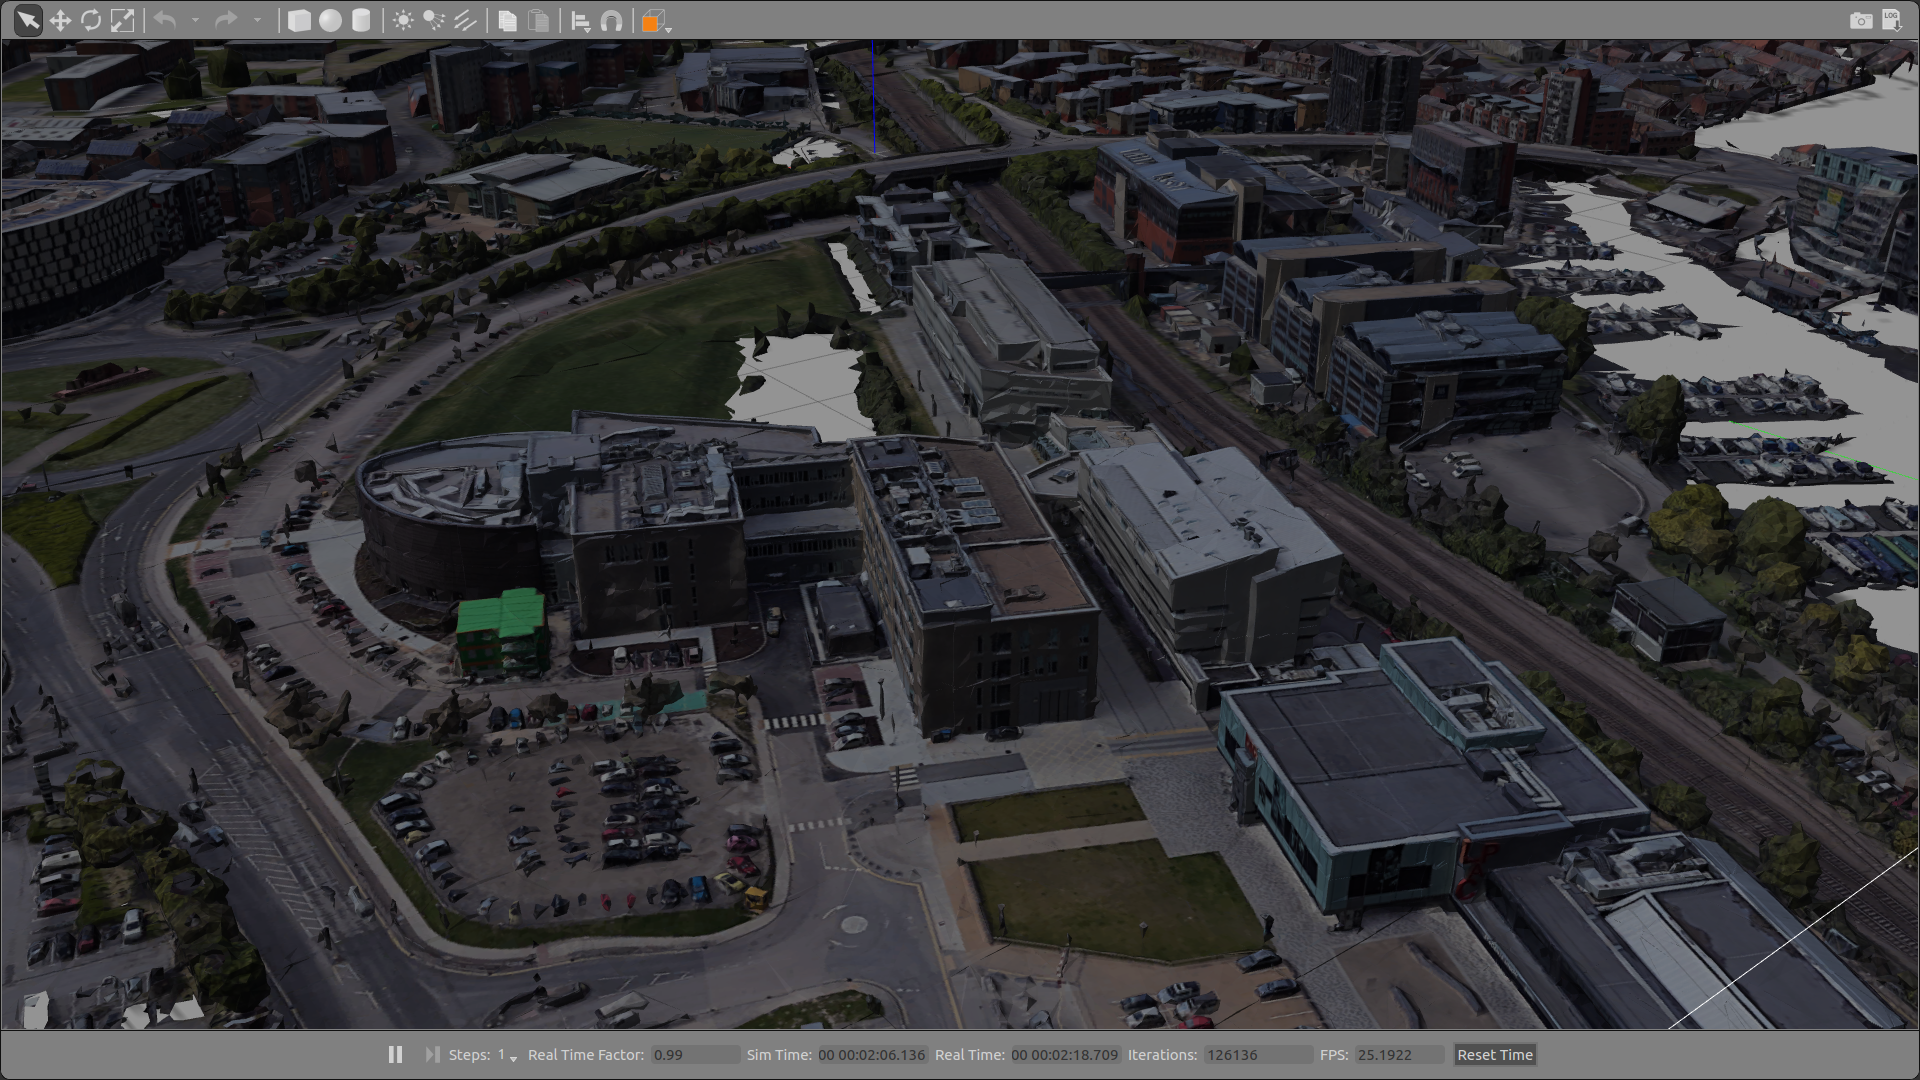
\includegraphics[width=\textwidth]{figs_sim/INBLincoln_2.png}
		\caption{University of Lincoln's Gazebo simulation world}
		\label{fig:INB_world}
	\end{figure*}


	\begin{figure*}[h]
		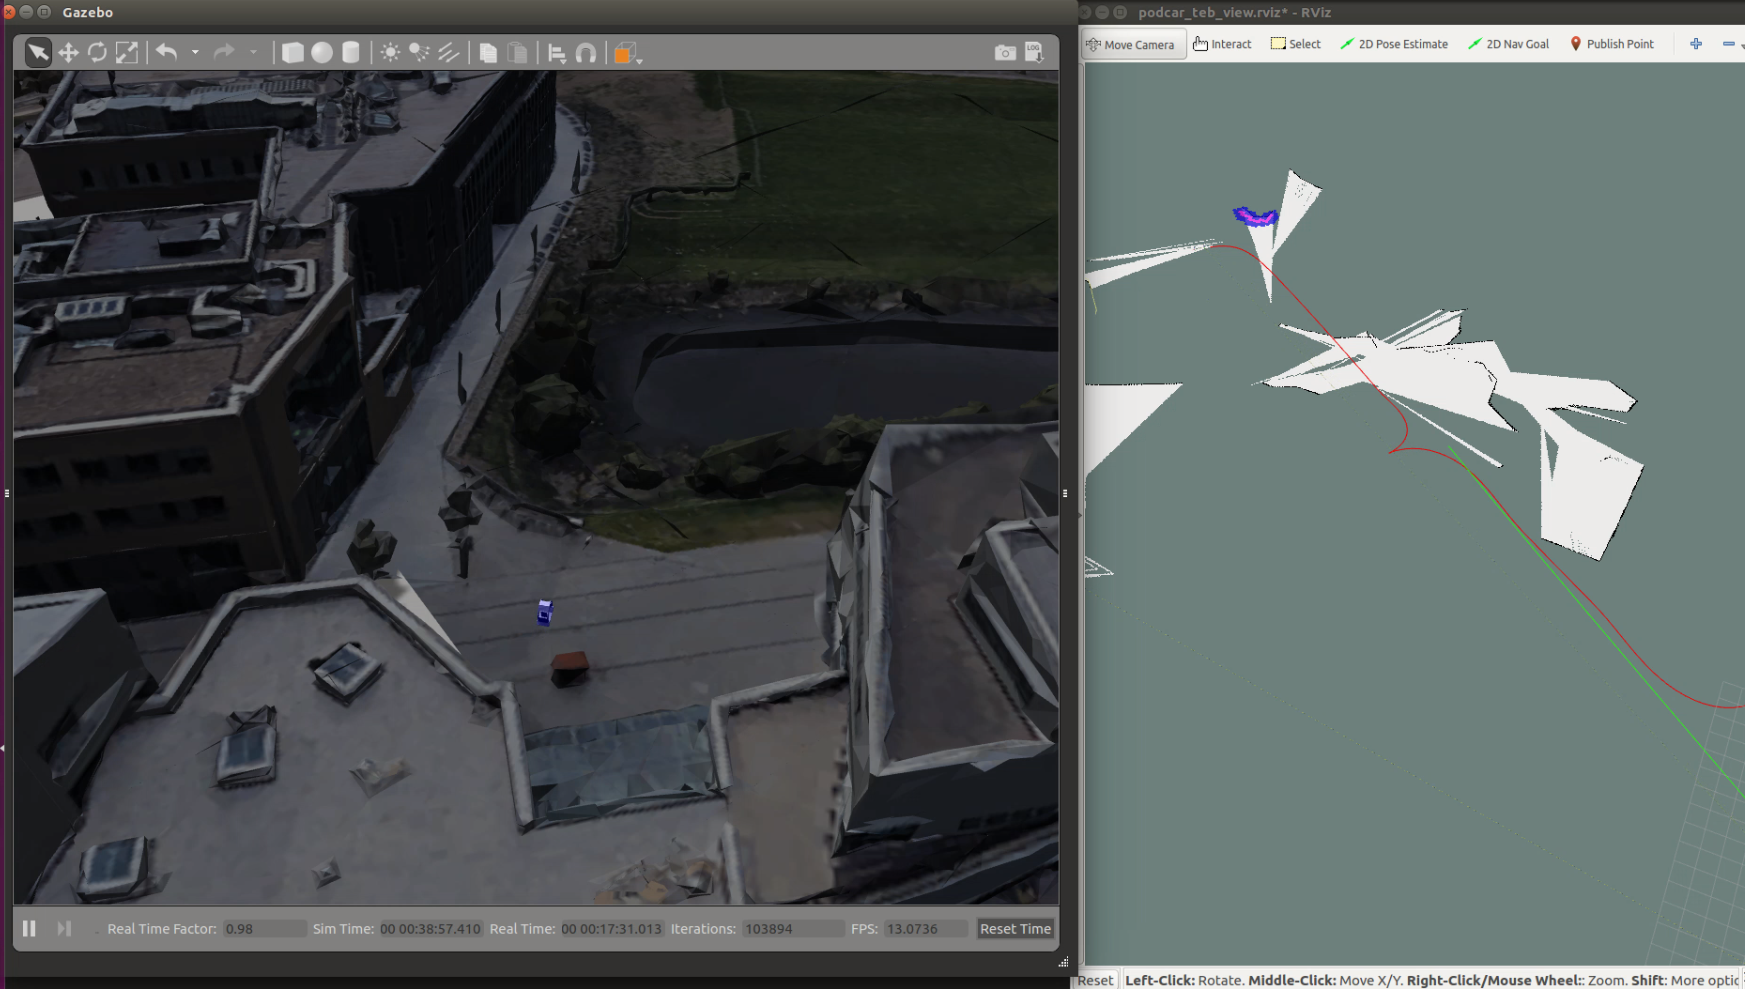
\includegraphics[width=\textwidth]{figs_sim/podcar_INB_teb.png}
		\caption{Podar in the University of Lincoln's Gazebo simulation world with Rviz TEB output}
		\label{fig:INB_teb}
	\end{figure*}

\section{Path planning and control (movebase)}

Front-wheel-steering means that the front two wheels are used to steer the vehicle, with the rear wheels trailing and-or powering the vehicle.  Ackermann steering is a special case of front-wheel-steering, in which the front wheels are connected to a tracking rod via two shorter steering arms arranged so that the two steering arms form a triangle with the center point of the vehicle’s rear axle when the wheels are facing forwards.  This results (TODO cite proof) in the front wheels forming the correct angles (which are different from each other) needed for the vehicle to drive in circular segments, with the circle radius determined by the steering angle.   Vehicles whose possible driving motions are of this form are called Dubins Cars if they can drive only forwards, or Reeds-Shepp cars if they can drive forwards and reverse. ubins and Reeds-Shepp cars have possible driving trajectories from pose A to pose B which consist of at most one circle arc segment and two straight lines to and from it. The donor podcar is a Reeds-Shepp car with Ackermann steering.

    \begin{figure}[h]
      \includegraphics[width=\columnwidth]{hardware/ackermann1.png}
      \caption{Ackermann steering (Source: Wikipedia; Ackermann Steering; Creative Commons.}
      \label{fig:ackermann1}
    \end{figure}

    \begin{figure}[h]
      \includegraphics[width=\columnwidth]{hardware/ackermann2.png}
      \caption{Ackermann steering (Source: Wikipedia; Ackermann Steering; Creative Commons.}
      \label{fig:ackermann1}
    \end{figure}

The values for parameters such as minimum turning radius were calculated from the technical specifications of the base vehicle \cite{shopriderflagship}.

Move Base is a set of ROS nodes that are standard for controlling robots via ROS. It enforces
conventions for being able to send messages to controllers, for example the use of Twist
messages. These messages are made up of 6 floats, the first 3 representing linear velocity in
each axis (x, y and z; forward, left and up) with the latter 3 representing angular velocity in
the same space. Move Base requires the robot to move with these given velocities when a
Twist message is published to the /cmd vel topic (Marder-Eppstein, 2018). These standards
ensure compatibility between packages, making the addition of existing packages to a project
much easier.

Twist messages, however, don’t apply to all robots. For example, the vast majority of robots
aren’t able to move directly up in the world, so the linear z component of the message is
ignored. A similar problem arises when considering ‘car-like’ steering, as they are unable to
inflict an angular velocity. In this case, the angular z component is instead taken to refer to the desired angle of the steerable wheels, which resolves the incompatibility problem provided
all nodes involved are aware of the difference. Alternatively, an intermediary node could be
introduced that calculates the wheel angle needed to make the robot turn at a given rate,
however this would be unnecessarily complex and wouldn’t have the desired effect if the
robot’s linear velocity was 0.

Fig. \ref{fig:sim_nodes} shows the complete ROS node configuration used during movebase, with the simulation backend.  When using the physical vehicle, simulation nodes are replaced by the physical vehicle nodes as described above.

\begin{figure}[h]
      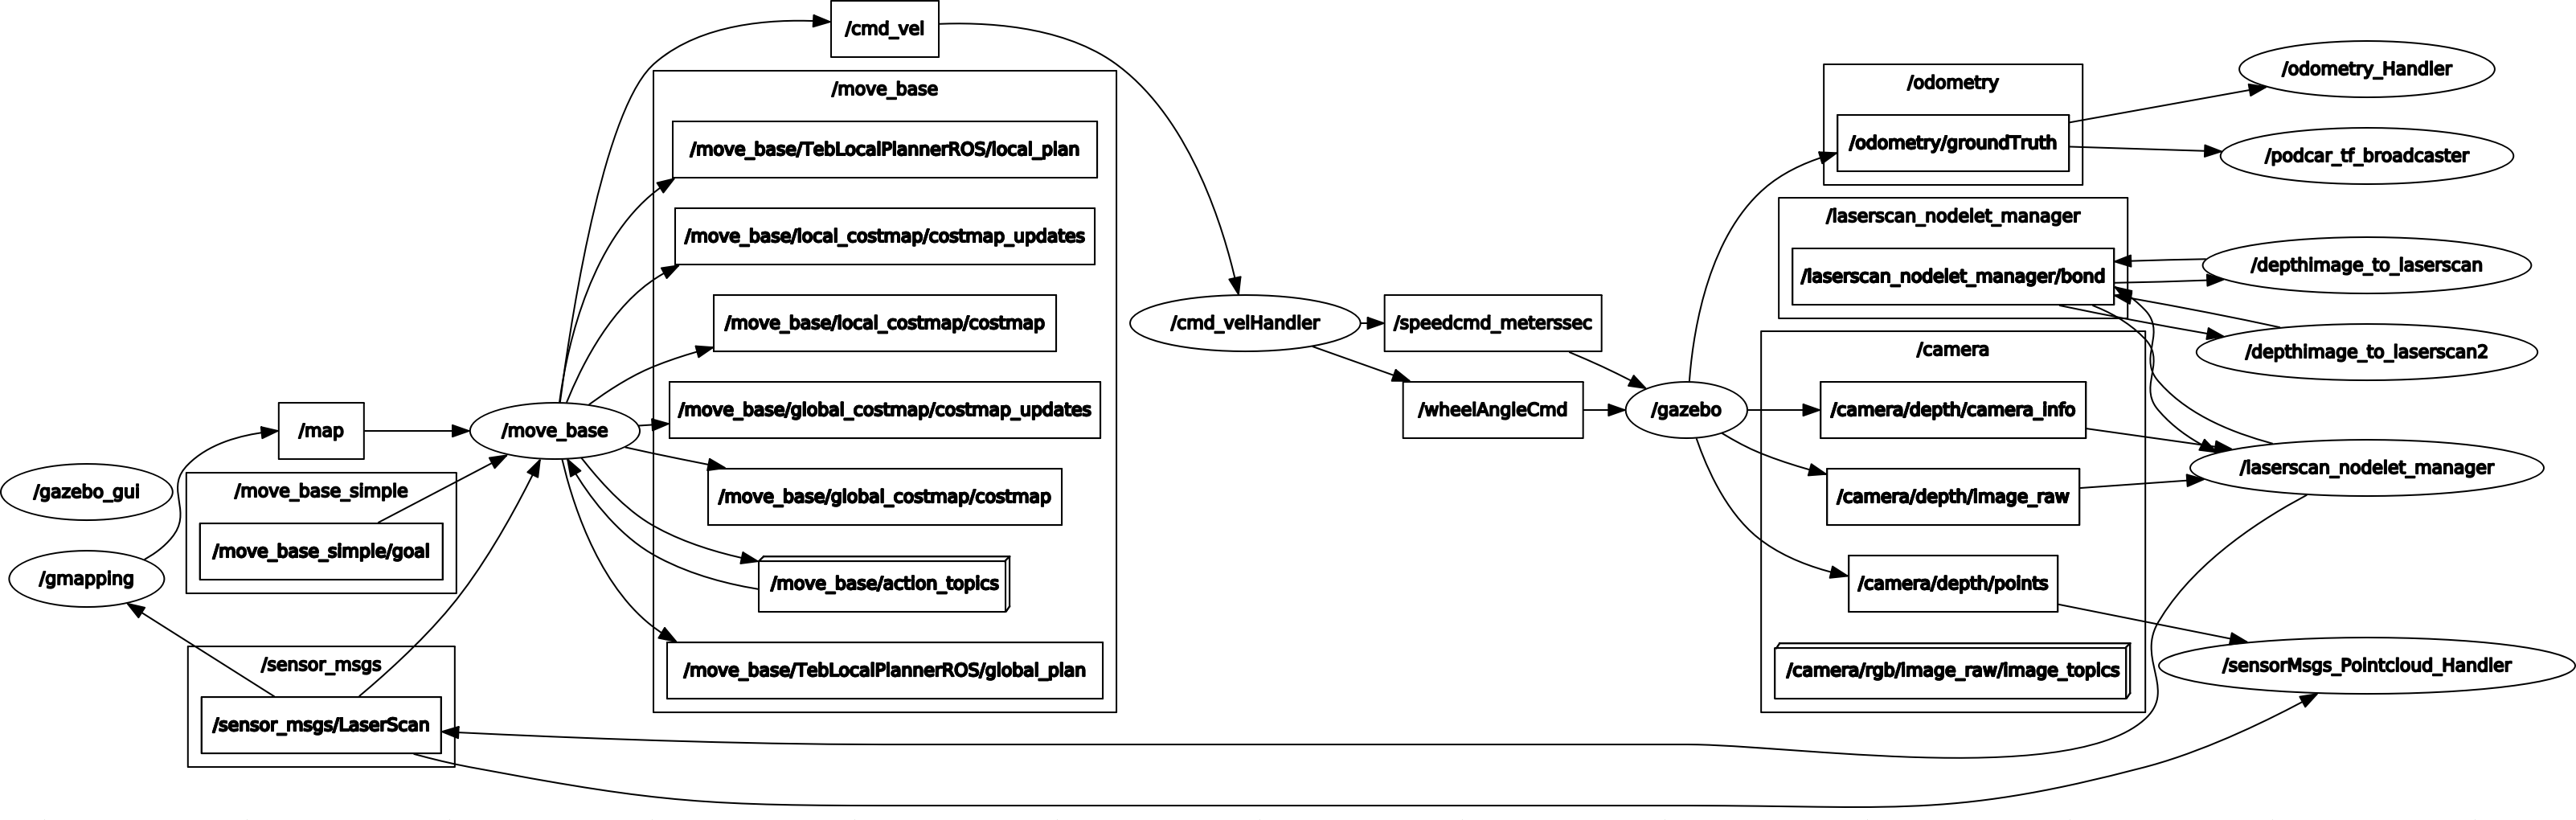
\includegraphics[width=\columnwidth]{figs_sim/sim_movebase_nodes.png}
      \caption{ROS nodes used in simulation under movebase control.}
      \label{fig:sim_movebase_nodes}
\end{figure}

\section{Localisation and mapping system}

gmapping -- current

TODO

    
\section{Discussion}
We hope that the platform will be useful...

\section{Future work}

\subsection{Depth camera option}

\subsection{Motor controller with OSMC}



    
\section{Acknowledgments}
This project has received funding from EU H2020 interACT: Designing cooperative interaction of automated vehicles with other road users in mixed traffic environments under grant agreement No 723395. Thanks to Jacob Lord for creating the vehicle graphical mesh model, Yao Chen for scoping Dubins path methods and the mechanical design, Gabriel Walton for scoping simulation tools, Yicheng Zhang for helping with the 3D printer and many other useful tools for the PCB board.
    
    
    
\bibliographystyle{plain}
\bibliography{podcar}
    



\end{document}








